\ifx\wholebook\relax \else
% ------------------------

\documentclass[b5paper]{article}
\usepackage[nomarginpar
  %, margin=.5in
]{geometry}

\addtolength{\oddsidemargin}{-0.05in}
\addtolength{\evensidemargin}{-0.05in}
\addtolength{\textwidth}{0.1in}

\usepackage[en]{../../../prelude}

\setcounter{page}{1}

\begin{document}

\title{Imperative delete for red-black tree}

\author{Xinyu LIU
\thanks{{\bfseries Xinyu LIU} \newline
  Email: liuxinyu95@gmail.com \newline}
  }

\maketitle
\fi

\markboth{Red-black tree}{Elementary Algorithms}

\ifx\wholebook\relax
\chapter{Imperative delete for red-black tree}
\numberwithin{Exercise}{chapter}
\fi

\index{Red-black tree!Imperative delete}

We need handle more cases for imperative $delete$ than $insert$. To resume balance after cutting off a node fro the red-black tree, we perform rotations and re-coloring. When delete a black node, rule 5 will be violated because the number of black nodes along the path through that node reduces by one. We introduce `doubly-black' to maintain the number of black nodes unchanged. Below example program adds `doubly black' to the color definition:

\lstset{frame = single}
\begin{lstlisting}[language = Bourbaki]
data Color {RED, BLACK, DOUBLY_BLACK}
\end{lstlisting}

When delete a node, we re-use the binary search tree $delete$ in the first step, then further fix the balance if the node is black.

\begin{algorithmic}[1]
\Function{Delete}{$T, x$}
  \State $p \gets$ \Call{Parent}{$x$}
  \State $q \gets$ NIL
  \If{\Call{Left}{$x$} = NIL}
    \State $q \gets$ \Call{Right}{$x$}
    \State \textproc{Replace}($x$, \Call{Right}{$x$}) \Comment{replace $x$ with its right sub-tree}
  \ElsIf{\Call{Right}{$x$} = NIL}
    \State $q \gets$ \Call{Left}{$x$}
    \State \textproc{Replace}($x$, \Call{Left{$x$}}) \Comment{replace $x$ with its left sub-tree}
  \Else
    \State $y \gets$ \textproc{Min}(\Call{Right}{$x$})
    \State $p \gets$ \Call{Parent}{$y$}
    \State $q \gets$ \Call{Right}{$y$}
    \State \Call{Key}{$x$} $\gets$ \Call{Key}{$y$}
    \State copy data from $y$ to $x$
    \State \textproc{Replace}($y$, \Call{Right}{$y$}) \Comment{replace $y$ with its right sub-tree}
    \State $x \gets y$
  \EndIf
  \If{\Call{Color}{$x$} = BLACK}
    \State $T \gets$ \textproc{Delete-Fix}($T$, \Call{Make-Black}{$p$, $q$}, $q$ = NIL?)
  \EndIf
  \State release $x$
  \State \Return $T$
\EndFunction
\end{algorithmic}

\textproc{Delete} takes the root $T$ and the node $x$ to be deleted as the parameters. $x$ can be located through $lookup$. If $x$ has an empty sub-tree, we cut off $x$, then replace it with the other sub-tree $q$. Otherwise, we locate the minimum node $y$ in the right sub-tree of $x$, then replace $x$ with $y$. We cut off $y$ after that. If $x$ is black, we call \textproc{Make-Black}($p$, $q$) to maintain the blackness before further fixing.

\begin{algorithmic}[1]
\Function{Make-Black}{$p$, $q$}
  \If{$p$ = NIL and $q$ = NIL}
    \State \Return NIL \Comment{The tree was singleton}
  \ElsIf{$q$ = NIL}
    \State $n \gets$ Doubly Black NIL
    \State \Call{Parent}{$n$} $\gets p$
    \State \Return $n$
  \Else
    \State \Return \Call{Blacken}{$q$}
  \EndIf
\EndFunction
\end{algorithmic}

If both $p$ and $q$ are empty, we are deleting the only leaf from a singleton tree. The result is empty. If the parent $p$ is not empty, but $q$ is, we are deleting a black leaf. We use NIL to replace that black leaf. As NIL is already black, we change it to 'doubly black' NIL to maintain the blackness. Otherwise, if neither $p$ nor $q$ is empty, we call \textproc{Blacken}($q$). If $q$ is red, it changes to black; if $q$ is already black, it changes to doubly black. As the next step, we need eliminate the doubly blackness through tree rotations and re-coloring. There are three different cases (\cite{CLRS}, pp292). The doubly black node can be NIL or not in all the cases.

\textbf{Case 1}. {\em The sibling of the doubly black node is black, and it has a red sub-tree.} We can rotate the tree to fix the doubly black. There are 4 sub-cases, all can be transformed to a uniformed structure as shown in \cref{fig:del-case1}.

\begin{figure}[htbp]
   \centering
   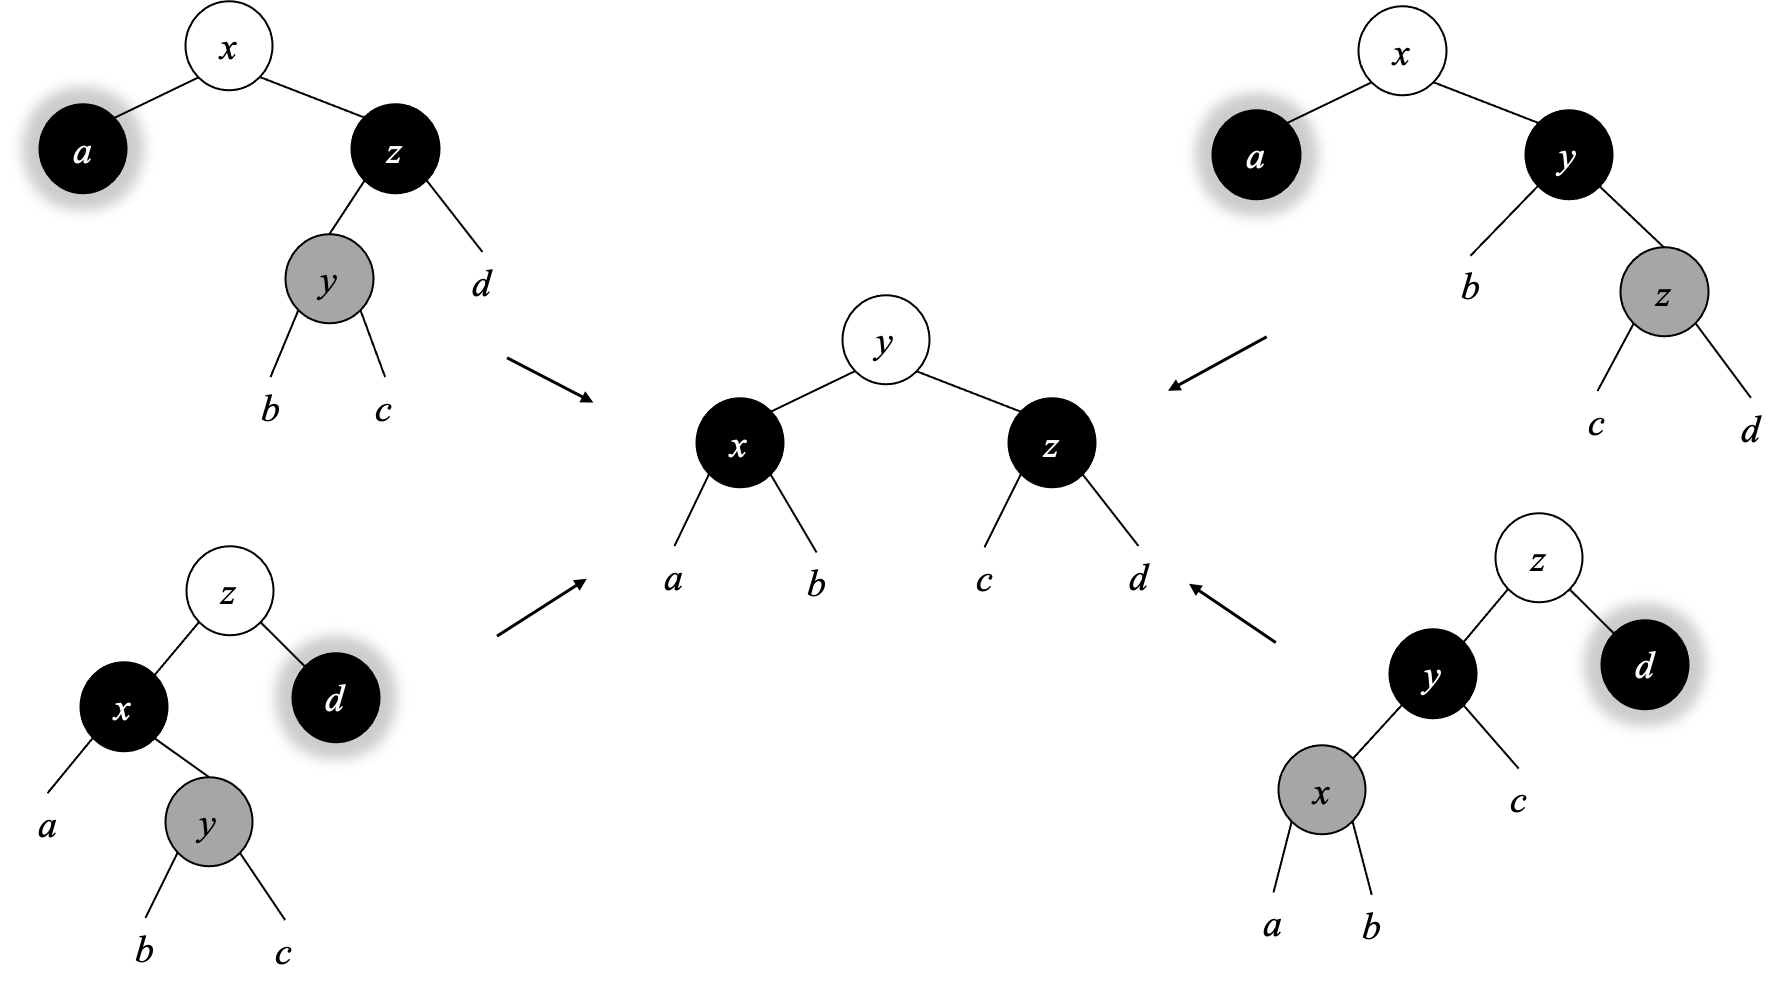
\includegraphics[scale=0.4]{../../../datastruct/tree/red-black-tree/img/del-case1}
   \caption{The doubly black node has a black sibling, and a red nephew. It can be fixed with a rotation.}
   \label{fig:del-case1}
\end{figure}

\begin{algorithmic}[1]
\Function{Delete-Fix}{$T$, $x$, $f$}
  \State $n \gets$ NIL
  \If{$f$ = True}  \Comment{$x$ is doubly black NIL}
    \State $n \gets x$
  \EndIf
  \If{$x$ = NIL} \Comment{Delete the singleton leaf}
    \State \Return NIL
  \EndIf
  \While{$x \neq T$ and \Call{Color}{$x$} $= \mathcal{B}^2$}
    \Comment{$x$ is doubly black, but not the root}
    \If{\Call{Sibling}{$x$} $\neq$ NIL} \Comment{The sibling is not empty}
        \State $s \gets$ \Call{Sibling}{$x$}
        \State ...
        \If{$s$ is black and \Call{Left}{$s$} is red}
          %\Comment{sibling: black, nephew: red}
          \If{$x = $ \textproc{Left}(\Call{Parent}{$x$})}
            \Comment{$x$ is the left}
            \State set $x$, \Call{Parent}{$x$}, and \Call{Left}{$s$} all black
            \State $T \gets$ \Call{Rotate-Right}{$T$, $s$}
            \State $T \gets$ \textproc{Rotate-Left}($T$, \Call{Parent}{$x$})
          \Else \Comment{$x$ is the right}
            \State set $x$, \Call{Parent}{$x$}, $s$, and \Call{Left}{$s$} all black
            \State $T \gets$ \textproc{Rotate-Right}($T$, \Call{Parent}{$x$})
          \EndIf
        \ElsIf{$s$ is black and \Call{Right}{$s$} is red}
          %\Comment{sibling: black, nephew: red}
          \If{$x = $ \textproc{Left}(\Call{Parent}{$x$})} \Comment{$x$ is the left}
            \State set $x$, \Call{Parent}{$x$}, $s$, and \Call{Right}{$s$} all black
            \State $T \gets$ \textproc{Rotate-Left}($T$, \Call{Parent}{$x$})
          \Else \Comment{$x$ is the right}
            \State set $x$, \Call{Parent}{$x$}, and \Call{Right}{$s$} all black
            \State $T \gets$ \Call{Rotate-Left}{$T$, $s$}
            \State $T \gets$ \textproc{Rotate-Right}($T$, \Call{Parent}{$x$})
          \EndIf
        \State ...
        \EndIf
    \EndIf
  \EndWhile
\EndFunction
\end{algorithmic}

\textbf{Case 2}. {\em The sibling of the doubly black is red.} We can rotate the tree to change the doubly black node to black. As shown in figure \cref{fig:del-case2}, change $a$ or $c$ to black. We can add this fixing to the previous implementation.

\begin{figure}[htbp]
  \centering
  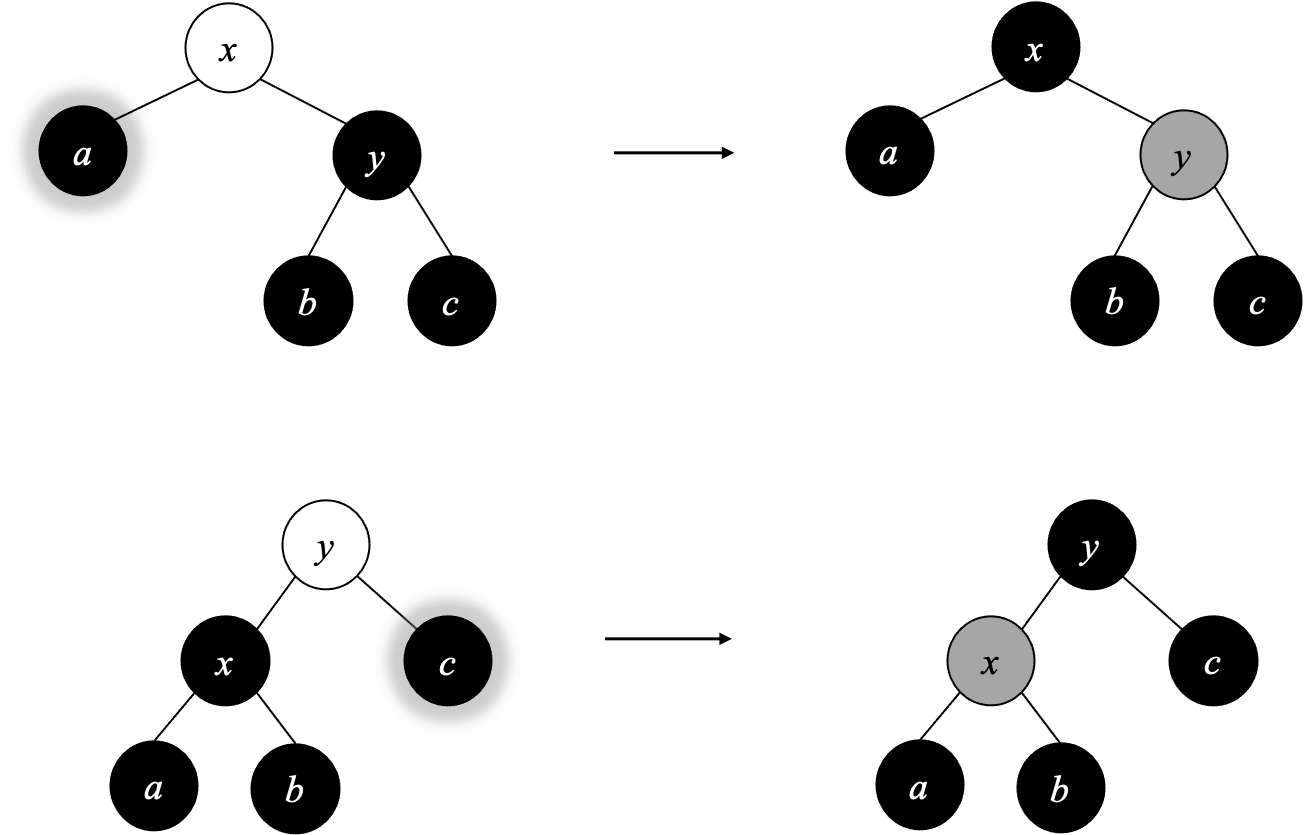
\includegraphics[scale=0.4]{../../../datastruct/tree/red-black-tree/img/del-case3}
  \caption{The sibling of the doubly black is red}
  \label{fig:del-case2}
\end{figure}

\begin{algorithmic}[1]
\Function{Delete-Fix}{$T$, $x$, $f$}
  \State $n \gets$ NIL
  \If{$f$ = True}  \Comment{$x$ is doubly black NIL}
    \State $n \gets x$
  \EndIf
  \If{$x$ = NIL} \Comment{Delete the singleton leaf}
    \State \Return NIL
  \EndIf
  \While{$x \neq T$ and \Call{Color}{$x$} $= \mathcal{B}^2$}
    %\Comment{$x$ isn't root and is doubly black}
    \If{\Call{Sibling}{$x$} $\neq$ NIL}
        \State $s \gets$ \Call{Sibling}{$x$}
        \If{$s$ is red}   \Comment{The sibling is red}
          \State set \Call{Parent}{$x$} red
          \State set $s$ black
          \If{$x = $ \textproc{Left}(\Call{Parent}{$x$})} \Comment{$x$ is the left}
            \State $T \gets$ \textproc{Rotate-Left}{$T$, \Call{Parent}{$x$}}
          \Else \Comment{$x$ is the right}
            \State $T \gets$ \textproc{Rotate-Right}{$T$, \Call{Parent}{$x$}}
          \EndIf
        \ElsIf{$s$ is black and \Call{Left}{$s$} is red}
          %\Comment{The sibling is black, a nephew is red}
          \State ...
        \EndIf
    \EndIf
  \EndWhile
\EndFunction
\end{algorithmic}

\textbf{Case 3}. {\em The sibling of the doubly black node, and its two sub-trees are all black.} In this case, we re-color the sibling to red, change the doubly black node back to black, then move the doubly blackness up to the parent. As shown in figure \cref{fig:del-case3}, there are two symetric sub-cases.

\begin{figure}[htbp]
  \centering
  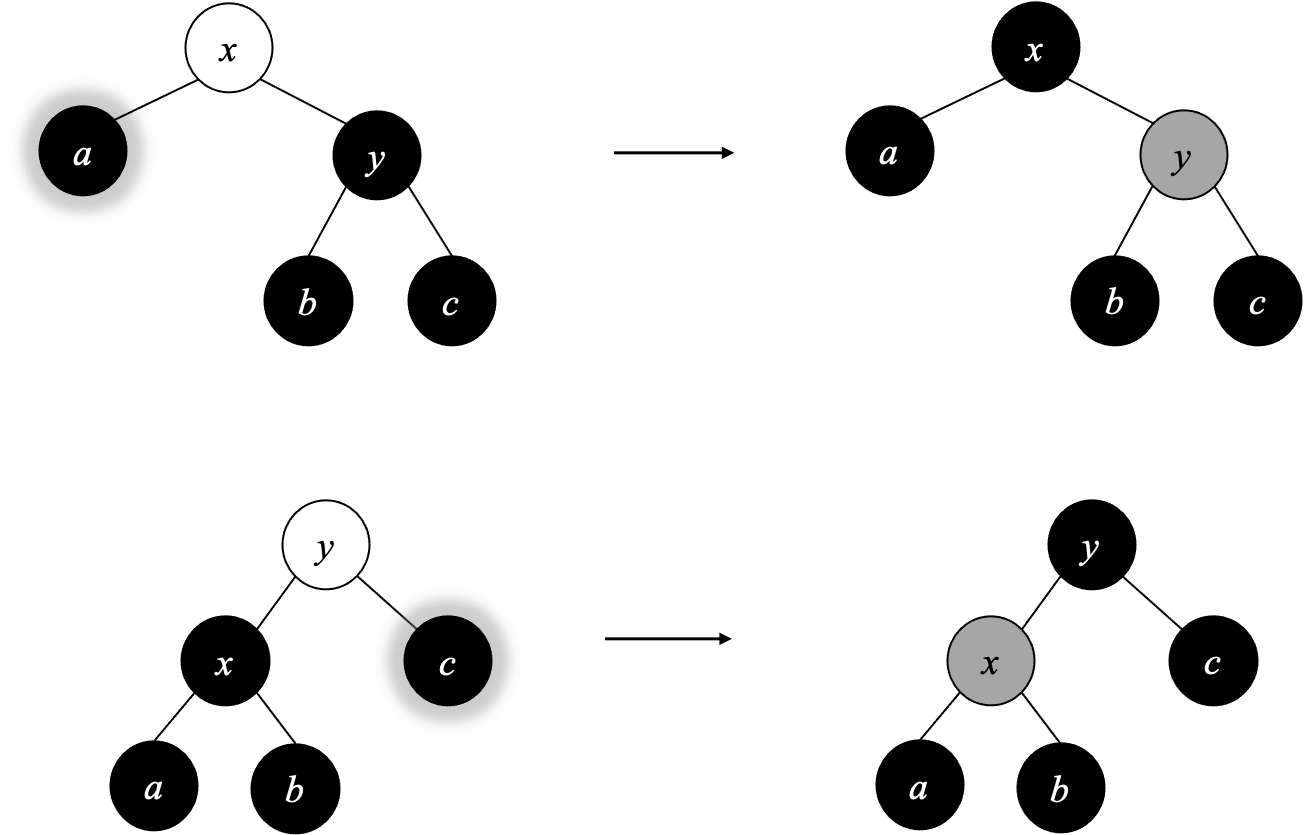
\includegraphics[scale=0.4]{../../../datastruct/tree/red-black-tree/img/del-case3}
  \caption{move the blackness up}
  \label{fig:del-case3}
\end{figure}

The sibling of the doubly black isn't empty in all above 3 cases. Otherwise, we change the doubly black node back to black, and move the blackness up. When reach the root, we force the root to be black to complete fixing. It also terminates if the doubly black node is eliminated after re-color in the midway. At last, if the doubly black node passed in is empty, we turn it back to normal NIL.

\begin{algorithmic}[1]
\Function{Delete-Fix}{$T$, $x$, $f$}
  \State $n \gets$ NIL
  \If{$f$ = True}  \Comment{$x$ is a doubly black NIL}
    \State $n \gets x$
  \EndIf
  \If{$x$ = NIL} \Comment{Delete the singleton leaf}
    \State \Return NIL
  \EndIf
  \While{$x \neq T$ and \Call{Color}{$x$} $= \mathcal{B}^2$}
    %\Comment{$x$ isn't root and is doubly black}
    \If{\Call{Sibling}{$x$} $\neq$ NIL} \Comment{The sibling is not empty}
        \State $s \gets$ \Call{Sibling}{$x$}
        \If{$s$ is red} \Comment{The sibling is red}
          \State set \Call{Parent}{$x$} red
          \State set $s$ black
          \If{$x = $ \textproc{Left}(\Call{Parent}{$x$})} \Comment{$x$ is the left}
            \State $T \gets$ \textproc{Rotate-Left}{$T$, \Call{Parent}{$x$}}
          \Else \Comment{$x$ is the right}
            \State $T \gets$ \textproc{Rotate-Right}{$T$, \Call{Parent}{$x$}}
          \EndIf
        \ElsIf{$s$ is black and \Call{Left}{$s$} is red}
          %\Comment{The sibling is black, a nephew is red}
          \If{$x = $ \textproc{Left}(\Call{Parent}{$x$})}
            \Comment{$x$ is the left}
            \State set $x$, \Call{Parent}{$x$}, and \Call{Left}{$s$} all black
            \State $T \gets$ \Call{Rotate-Right}{$T$, $s$}
            \State $T \gets$ \textproc{Rotate-Left}($T$, \Call{Parent}{$x$})
          \Else \Comment{$x$ is the right}
            \State set $x$, \Call{Parent}{$x$}, $s$, and \Call{Left}{$s$} all black
            \State $T \gets$ \textproc{Rotate-Right}($T$, \Call{Parent}{$x$})
          \EndIf
        \ElsIf{$s$ is black and \Call{Right}{$s$} is red}
          %\Comment{The sibling is black, a nephew is red}
          \If{$x = $ \textproc{Left}(\Call{Parent}{$x$})}
            \Comment{$x$ is the left}
            \State set $x$, \Call{Parent}{$x$}, $s$, and \Call{Right}{$s$} all black
            \State $T \gets$ \textproc{Rotate-Left}($T$, \Call{Parent}{$x$})
          \Else \Comment{$x$ is the right}
            \State set $x$, \Call{Parent}{$x$}, and \Call{Right}{$s$} all black
            \State $T \gets$ \Call{Rotate-Left}{$T$, $s$}
            \State $T \gets$ \textproc{Rotate-Right}($T$, \Call{Parent}{$x$})
          \EndIf
        \ElsIf{$s$, \Call{Left}{$s$}, and \Call{Right}{$s$} are all black}
          %\Comment{The sibling and sub-trees are all black}
          \State set $x$ black
          \State set $s$ red
          \State \textproc{Blacken}(\Call{Parent}{$x$})
          \State $x \gets$ \Call{Parent}{$x$}
        \EndIf
    \Else \Comment{move the blackness up}
      \State set $x$ black
      \State \textproc{Blacken}(\Call{Parent}{$x$})
      \State $x \gets$ \Call{Parent}{$x$}
    \EndIf
  \EndWhile
  \State set $T$ black
  \If{$n \neq$ NIL}
    \State replace $n$ with NIL
  \EndIf
  \State \Return $T$
\EndFunction
\end{algorithmic}

When fixing, we pass in the root $T$, the node $x$ (can be doubly black), and a flag $f$. The flag is true if $x$ is doubly black NIL. We record it with $n$, and replace $n$ with the normal NIL after fixing.

Below is the example program implements delete:

\begin{lstlisting}[language = Bourbaki]
Node del(Node t, Node x) {
    if x == null then return t
    var parent = x.parent;
    Node db = null;        //doubly black

    if x.left == null {
        db = x.right
        x.replaceWith(db)
    } else if x.right == null {
        db = x.left
        x.replaceWith(db)
    } else {
        var y = min(x.right)
        parent = y.parent
        db = y.right
        x.key = y.key
        y.replaceWith(db)
        x = y
    }
    if x.color == Color.BLACK {
        t = deleteFix(t, makeBlack(parent, db), db == null);
    }
    remove(x)
    return t
}
\end{lstlisting}

Where \texttt{makeBlack} checks if the node changes to doubly black, and handles the special case of doubly black NIL.

\begin{lstlisting}[language = Bourbaki]
Node makeBlack(Node parent, Node x) {
    if parent == null and x == null then return null
    return if x == null
        then replace(parent, x, Node(0, Color.DOUBLY_BLACK))
        else blacken(x)
}
\end{lstlisting}

The function \texttt{replace(parent, x, y)} replaces the child of the \texttt{parent}, which is \texttt{x}, with \texttt{y}.

\begin{lstlisting}[language = Bourbaki]
Node replace(Node parent, Node x, Node y) {
    if parent == null {
        if y != null then y.parent = null
    } else if parent.left == x {
        parent.setLeft(y)
    } else {
        parent.setRight(y)
    }
    if x != null then x.parent = null
    return y
}
\end{lstlisting}

The function \texttt{blacken(node)} changes the red node to black, and the black node to doubly black:

\begin{lstlisting}[language = Bourbaki]
Node blacken(Node x) {
    x.color = if isRed(x) then Color.BLACK else Color.DOUBLY_BLACK
    return x
}
\end{lstlisting}

Below example program implements the fixing:

\begin{lstlisting}[language = Bourbaki]
Node deleteFix(Node t, Node db, Bool isDBEmpty) {
    var dbEmpty = if isDBEmpty then db else null
    if db == null then return null    // delete the root
    while (db != t and db.color == Color.DOUBLY_BLACK) {
        var s = db.sibling()
        var p = db.parent
        if (s != null) {
            if isRed(s) {
                // the sibling is red
                p.color = Color.RED
                s.color = Color.BLACK
                t = if db == p.left then leftRotate(t, p)
                                    else rightRotate(t, p)
            } else if isBlack(s) and isRed(s.left) {
                // the sibling is black, and one sub-tree is red
                if db == p.left {
                    db.color = Color.BLACK
                    p.color  = Color.BLACK
                    s.left.color = p.color
                    t = rightRotate(t, s)
                    t = leftRotate(t, p)
                } else {
                    db.color = Color.BLACK
                    p.color  = Color.BLACK
                    s.color = p.color
                    s.left.color = Color.BLACK
                    t = rightRotate(t, p)
                }
            } else if isBlack(s) and isRed(s.right) {
                if (db == p.left) {
                    db.color = Color.BLACK
                    p.color  = Color.BLACK
                    s.color  = p.color
                    s.right.color = Color.BLACK
                    t = leftRotate(t, p)
                } else {
                    db.color = Color.BLACK
                    p.color  = Color.BLACK
                    s.right.color = p.color
                    t = leftRotate(t, s)
                    t = rightRotate(t, p)
                }
            } else if isBlack(s) and isBlack(s.left) and
                      isBlack(s.right) {
                // the sibling and both sub-trees are black.
                // move blackness up
                db.color = Color.BLACK
                s.color  = Color.RED
                blacken(p)
                db = p
            }
        } else { // no sibling, move blackness up
            db.color = Color.BLACK
            blacken(p)
            db = p
        }
    }
    t.color = Color.BLACK
    if (dbEmpty != null) { // change the doubly black nil to nil
        dbEmpty.replaceWith(null)
        delete dbEmpty
    }
    return t
}
\end{lstlisting}

Where \texttt{isBlack(x)} tests if a node is black, the NIL node is also black.

\begin{lstlisting}[language = Bourbaki]
Bool isBlack(Node x) = (x == null or x.color == Color.BLACK)

Bool isRed(Node x) = (x != null and x.color == Color.RED)
\end{lstlisting}

Before returning the final result, we check the doubly black NIL, and call the \texttt{replaceWith} function defined in \texttt{Node}.

\begin{lstlisting}[language = Bourbaki]
data Node<T> {
    //...
    void replaceWith(Node y) = replace(parent, this, y)
}
\end{lstlisting}

The program terminates when reach the root or the doubly blackness is eliminated. As we maintain the red-black tree balanced, the delete algorithm is bound to $O(\lg n)$ time for the tree of $n$ nodes.

\begin{Exercise}
\Question{Write a program to test if a tree satisfies the 5 red-black tree rules. Use this program to verify the red-black tree delete implementation.}
\end{Exercise}

\ifx\wholebook\relax \else
\begin{thebibliography}{99}

\bibitem{CLRS}
Thomas H. Cormen, Charles E. Leiserson, Ronald L. Rivest and Clifford Stein.
``Introduction to Algorithms, Second Edition''. ISBN:0262032937. The MIT Press. 2001

\end{thebibliography}

\expandafter\enddocument
\fi
